\section{UPPAAL}
When planning satellite missions it is important, that it can be guaranteed no major or unforeseen errors will occur. This may be done testing or by using a modelling tool capable of verifying, that the proposed actions are correct\cite{cs_smc}. Several such tools exists e.g. Kronos, and UPPAAL. For this project we will be considering UPPAAL, specifically the versions \gls{cora} and \gls{smc}, as they have been presented as the more relevant solutions for this project.
\ofx{Maybe move smc stuff}
Common for all versions of UPPAAL, is that; it has global decelerations, and templates. One model may have several templates, each with its own local decelerations. The template itself consists of one to many locations and edges, edges connects the locations and when activated indicates a chance in the current state.\\
Edges may be decorated with; selects, guards, synchronizations, and updates. Selects are used for introducing new temporary variables. Guards are used to ensure that an edge is not activated prematurely. Synchronizations are used for activating multiple edges across templates simultaneously. Finally updates are used to chance variable values, and to call functions written in declarations.\\
Locations can be given a name, and an invariant. An invariant must always be evaluated to true e.g. if a location have the invariant $time <= 5$, at time five there will be a chance of state.\\
Also common for the versions of UPPAAL, is that queries can be written i order to ensure sustain properties are upheld, such as; is some location reachable, and will time ever exceed some amount. To complement this there is an available simulator allowing the user to monitor the behaviour of their model, in the simulator the user can decide step by step what the model does, or generate a random trace.


\subsection{UPPAAL CORA}
UPPAAL \gls{cora} is a version of UPPAAL which uses priced timed automata \cite{cs_cora}. \Gls{cora} have previously been used to find cost-optimal solutions for the GomX-3 system\cite{gomx3}, and is therefore considered relevant for this case.
\Gls{cora} is considered relatively basic for UPPAAL, as it is one of the older versions, it is however fast relative to some of the newer versions. \Gls{cora} introduced the concept of cost, this means that when a template reaches certain locations, it may have some specified cost, this however is limited to be linear. In addition it is possible to generate the most cost optimal trace, the minimum cost. Or a query asking for a sustain state where the cost is under some specified amount.\\
This can be advantageous for modelling systems such as satellites where energy is an important and limited resource which can be represented by the cost. After running a query it is possible to extract a trace, which can be used to represent the generated schedule.


\subsection{UPPAAL SMC}
UPPAAL \gls{smc} is one of the newer versions of UPPAAL, it works with statistical model checking for more efficient analysis, as it avoids the exhaustive exploration of the state-space. This statistical exploration gives the added benefit of significantly less memory consumption\cite{cs_smc}, meaning that the computers physical memory is rarely the limit when running a query. This flexibility allows for \gls{smc} to be used for other subjects than verification such as planing\cite{cs_smc}. \\
In addition \gls{smc} have been updated so that it can handle non linear cost and differential equations which makes it possible to implement \gls{kibam}.

After having run a simulation query, it is possible to get a graph illustrating the result of running the simulations. In \cref{fig:simab} we see two variable which have been simulated five times for $15.000$ units of time, this will be useful for monitoring the battery energy levels over time.

\begin{figure}[h]
	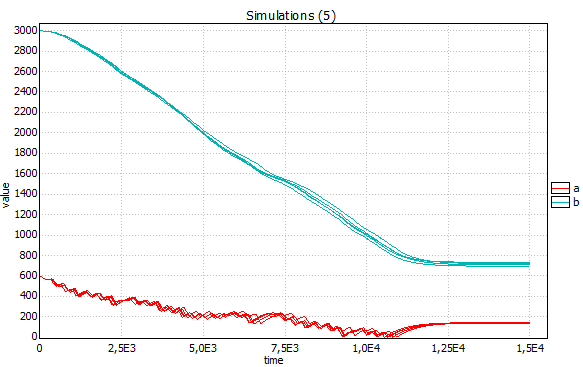
\includegraphics[width=\textwidth]{graphics/simab.png}
	\label{fig:simab}
	\caption{Five simulations of the value of two variables \uppVar{a, b} over time}
\end{figure}

Also it is possible to run probabilities queries, these answers the question; \textit{"What is the probability that some condition will be fulfilled?"}. An example of this can be seen in \cref{fig:pra300}, where we have run the probability that our variable \uppVar{a} will fall below $300$ within time $7200$. \Gls{smc} have then run this by randomly simulating the models behaviour until it with some certainty, within a specified margin of error, knows the chance of the property being true.\\
\Cref{fig:pra300} shows that prior to time $4120$ there are no chance of \uppVar{a} being under $300$, and at time $4520$ it will with certainty be under $300$. For this query it was specified that a $5\%$ uncertainty was acceptable, this resulted in the result seen in \cref{fig:pra300pct} which shows that \gls{smc} was $~90\% - 100\%$ certain \uppVar{a} would fall below $300$. The certainty parameter can be modified to become more precise, at the cost of run time as it will have to run more simulations in order to ensure the correct probability. Using the probability query also allow  for several other types graphs such as probability distribution and frequency histogram.

\begin{figure}[h]
	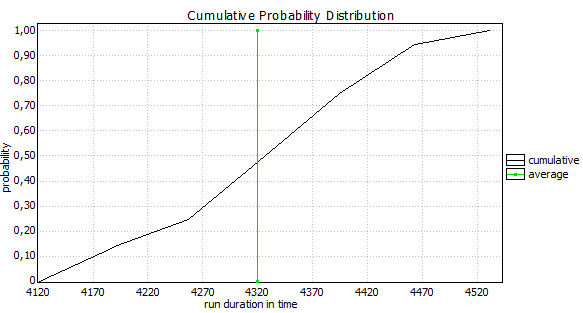
\includegraphics[width=\textwidth]{graphics/pra300.png}
	\label{fig:pra300}
	\caption{Probability over time that the value of (a) will fall under 300}
\end{figure}

\begin{figure}[h]
	\centering
	
\includegraphics[width=8cm]{graphics/pra300pct.png}
	\label{fig:pra300pct}
	\caption{Initial result of running a probability query}
\end{figure}


